\documentclass[10pt,letterpaper]{article} 
\usepackage{tikz}
\usepackage{tools}
\usepackage{enumitem}
\usepackage{listings}
\lstset{language=Python}
%\lstset{frame=lines}
%\lstset{caption={Insert code directly in your document}}
\lstset{label={lst:code_direct}}
\lstset{basicstyle=\footnotesize}

%\usepackage{graphicx}‎‎
%\usefonttheme{serif}‎
%\usepackage{ptext}‎
%\usepackage{xepersian}
%\settextfont{B Nazanin}
\usepackage{lipsum}
\setlength{\parindent}{0pt}
\newcommand{\pf}{$\blacksquare$}

\newcommand{\Span}{\text{Span}}
\newcommand{\NF}{\text{NF}}
\newcommand{\EDFA}{\text{EDFA}}
\newcommand{\ASE}{\text{ASE}}

\newcommand{\bns}{\textit{broadcast-and-select}  architecture}
\newcommand{\Bns}{\textit{Broadcast-and-select} architecture}

\newcommand{\rns}{\textit{route-and-select} architecture}
\newcommand{\Rns}{\textit{Route-and-select} architecture}

\newcounter{QuestionNumber}
\setcounter{QuestionNumber}{1}

\newcommand{\temp}{{\color{red}{temp}}}

\newcommand{\Q}{
\textbf{Question \theQuestionNumber)}
\stepcounter{QuestionNumber}
}
\newcommand{\EX}{\Bbb E}
\newcommand{\nl}{\newline\newline}
\begin{document}
\large
\begin{center}
In the name of beauty

The 6th problem set of Optical Networks course
\hl
\end{center}
\Q

By making use of Bhandari's algorithm (an SPDP algorithm for finding more than one shortest path between two nodes), find two link-disjoint shortest paths between nodes 1 and 8. \textbf{All the links have a cost equal to 1.}
%\picnocapt{PS6_Q1.pdf}{130mm}
\begin{figure}[h!]
\centering
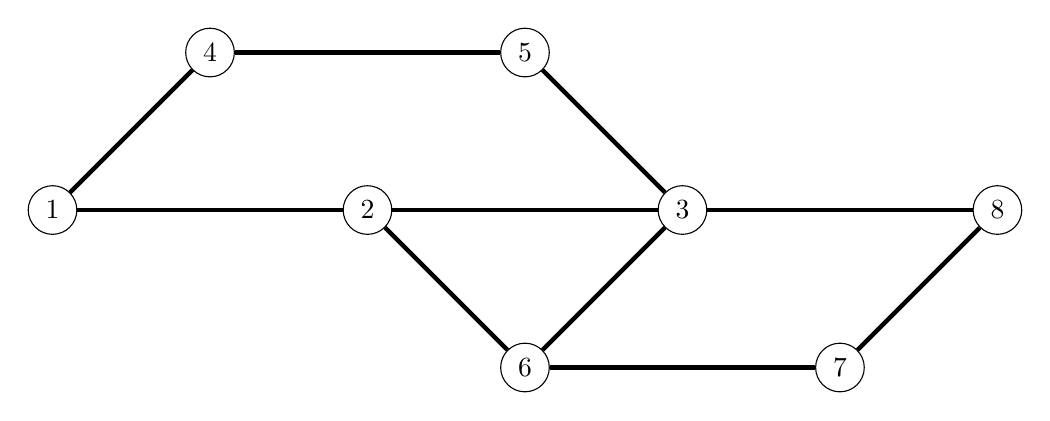
\begin{tikzpicture}

\node [draw, shape=circle] (n1) at (-2,0) {1};
\node[draw,shape=circle](n2) at (2,0){2};
\node[draw,shape=circle](n3) at (6,0){3};
\node[draw,shape=circle](n4) at (0,2){4};
\node[draw,shape=circle](n5) at (4,2){5};
\node[draw, shape=circle] (n6) at (4,-2) {6};
\node[draw, shape=circle] (n7) at (8,-2) {7};
\node[draw, shape=circle] (n8) at (10,0) {8};


\draw[ultra thick] (n1) -- (n2);
\draw[ultra thick] (n3) -- (n2);
\draw[ultra thick] (n3) -- (n8);
\draw[ultra thick] (n1) -- (n4);
\draw[ultra thick] (n5) -- (n4);
\draw[ultra thick] (n3) -- (n5);
\draw[ultra thick] (n2) -- (n6);
\draw[ultra thick] (n6) -- (n7);
\draw[ultra thick] (n6) -- (n3);
\draw[ultra thick] (n8) -- (n7);
%\draw[ultra thick] (n1) --node [below] {1} (n3);
%\draw[ultra thick] (n2) --node [below] {1} (n3);
%\draw[ultra thick] (n1) --node [below,left] {1} (n4);
%\draw[ultra thick] (n7) --node [below,left] {2} (n6);
%\draw[ultra thick] (n5) --node [below,left] {1} (n6);
%\draw[ultra thick] (n5) --node [below,left] {1} (n3);
%\draw[ultra thick] (n4) --node [below] {1} (n7);
%\draw[ultra thick] (n3) --node [below] {1} (n6);


\end{tikzpicture}
\end{figure}

\Q

Solve the following ILP problem:
\eqn{
&\text{Objective}\quad \max \quad 12x_1+10x_2
\\&\text{Constraints}\begin{cases}
2x_1+3x_3\le 30
\\3x_1+2x_2\le 24
\\x_1=0,1,2,\cdots\text{ (integer value)}
\\x_2=0,1,2,\cdots\text{ (integer value)}
\end{cases}
}{}

\Q

In the following network, in case the link (4,5) is removed:

a. Find the shortest path from node 1 to node 6.

b. Find the shortest path from node 2 to node 6.

\picnocapt{PS6_Q3.png}{100mm}
\newpage
\Q
Find two disjoint paths from node 1 to node 12 to minimize the total costs of the paths in the following networks using:
\begin{enumerate}[label=\alph*-]
\item
Bhandari's algorithm.
\item
Suurballe's algorithm.
\end{enumerate}
What is the difference between the solutions of the two algorithms?

\begin{figure}[h!]
\centering
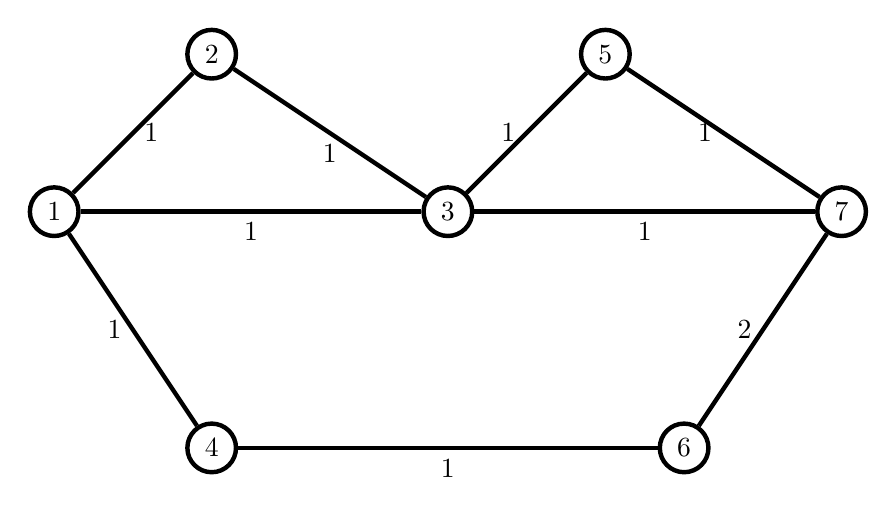
\begin{tikzpicture}

\node [draw, shape=circle,ultra thick] (n1) at (-1,0) {1};
\node[draw,shape=circle,ultra thick](n2) at (1,2){2};
\node[draw,shape=circle,ultra thick](n3) at (4,0){3};
\node[draw,shape=circle,ultra thick](n4) at (1,-3){4};
\node[draw,shape=circle,ultra thick](n5) at (6,2){5};
\node[draw, shape=circle,ultra thick] (n6) at (9,0) {7};
\node[draw, shape=circle,ultra thick] (n7) at (7,-3) {6};


\draw[ultra thick] (n1) --node [below,right] {1} (n2);
\draw[ultra thick] (n1) --node [below] {1} (n3);
\draw[ultra thick] (n2) --node [below] {1} (n3);
\draw[ultra thick] (n1) --node [below,left] {1} (n4);
\draw[ultra thick] (n7) --node [below,left] {2} (n6);
\draw[ultra thick] (n5) --node [below,left] {1} (n6);
\draw[ultra thick] (n5) --node [below,left] {1} (n3);
\draw[ultra thick] (n4) --node [below] {1} (n7);
\draw[ultra thick] (n3) --node [below] {1} (n6);


\end{tikzpicture}
\end{figure}


\Q

Consider an SRLG configuration consisting of two links, where the only point in common between the two links is an amplifier hut somewhere in the middle of the two links, i.e., the links cross (see figure below). How can such an SRLG be handled in an SPDP algorithm to ensure that the two crossing links are not treated as being diverse?
\begin{figure}[h!]
\centering
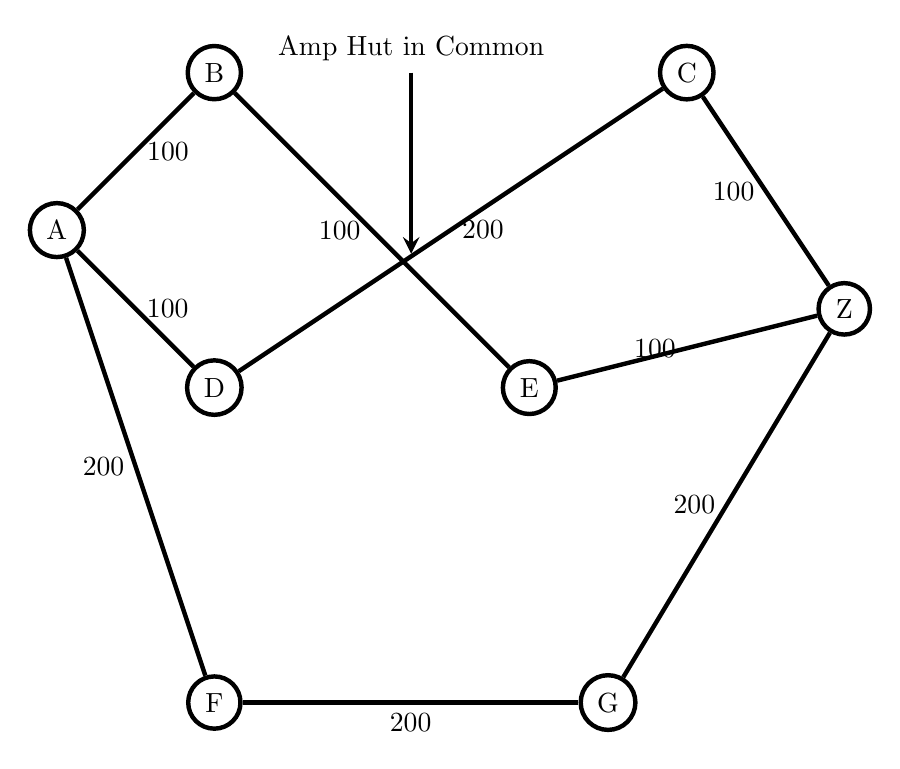
\begin{tikzpicture}

\node [draw, shape=circle,ultra thick] (n1) at (-1,0) {A};
\node[draw,shape=circle,ultra thick](n2) at (1,2){B};
\node[draw,shape=circle,ultra thick](n3) at (1,-2){D};
\node[draw,shape=circle,ultra thick](n4) at (7,2){C};
\node[draw,shape=circle,ultra thick](n5) at (5,-2){E};
\node[draw, shape=circle,ultra thick] (n6) at (9,-1) {Z};
\node[draw,shape=circle,ultra thick](n7) at (1,-6){F};
\node[draw,shape=circle,ultra thick](n8) at (6,-6){G};

\draw[ultra thick] (n1) --node [below,right] {100} (n2);
\draw[ultra thick] (n1) --node [below,right] {100} (n3);
\draw[ultra thick] (n3) --node [below,right] {200} (n4);
\draw[ultra thick] (n2) --node [below,left] {100} (n5);
\draw[ultra thick] (n4) --node [below,left] {100} (n6);
\draw[ultra thick] (n5) --node [below,left] {100} (n6);
\draw[ultra thick] (n1) --node [below,left] {200} (n7);
\draw[ultra thick] (n7) --node [below] {200} (n8);
\draw[ultra thick] (n8) --node [below,left] {200} (n6);

\draw[ ultra thick,color = black,-stealth] (3.5,2) -- node[]{}  (3.5,-0.3) ;

\draw[ultra thick] (3.5,2) --node [above] {Amp Hut in Common} (3.5,2);

\end{tikzpicture}
\end{figure}

\end{document}




